\documentclass[11pt]{article}
\usepackage{color}
\usepackage{amsmath,amsthm,amssymb,multirow,paralist}
\usepackage[margin=0.8in]{geometry}
\usepackage{hyperref}
\usepackage{graphicx}

\begin{document}

\begin{center}
{\Large \textbf{10-Year Risk of Coronary Hearty Disease}

\vspace{10pt}

Project Final Report}

\vspace{10pt}

\textit{Team Members: Yu Pei}
\end{center}

\begin{abstract}
  This project addresses the urgent need to predict 10-year Coronary Heart Disease (CHD) risk using a comprehensive set of variables including demographics, lifestyle factors, medical history, and biomarkers. Motivated by the staggering global death toll due to heart diseases, especially in developed nations, the objective is to empower healthcare providers with a machine learning model for accurate risk assessment and personalized interventions. Leveraging Support Vector Machines (SVM), Logistic Regression, and Decision Trees, the model not only surpasses traditional risk assessment methods but also provides actionable insights. Results demonstrate significantly improved CHD risk prediction, facilitating early interventions and efficient allocation of healthcare resources, leading to a tangible reduction in CHD-related morbidity and mortality rates.
\end{abstract}
\section{Introduction}
\subsection{Project Objectives}
\text The objective of this project is to develop a machine learning model capable of predicting the 10-year risk of Coronary Heart Disease (CHD) based on demographic, lifestyle, medical history, and biomarker variables. The project addresses the crucial need for early diagnosis and personalized preventive interventions in reducing the morbidity and mortality rates associated with cardiovascular diseases, particularly CHD. By leveraging machine learning techniques, the model aims to assist healthcare providers in accurately assessing CHD risk for individual patients, thereby improving patient outcomes.
\subsection{Datasets}
\text The dataset used for this project is publicly available on the Kaggle website and is derived from an ongoing cardiovascular study conducted on residents of Framingham, Massachusetts. The dataset comprises various features such as sex, age, smoking habits, medication usage, medical history (including stroke, hypertension, and diabetes), cholesterol levels, blood pressure, body mass index (BMI), heart rate, and glucose levels. The target variable for prediction is the 10-year risk of coronary heart disease (CHD), represented as binary labels ("1" for "Yes" and "0" for "No").
\begin{itemize}
    \item male: 0 = Female; 1 = Male
    \item age: Age at exam time.
    \item education: 1 = Some High School; 2 = High School or GED; 3 = Some College or Vocational School; 4 = College
    \item currentSmoker: 0 = nonsmoker; 1 = smoker
    \item cigsPerDay: number of cigarettes smoked per day (estimated average)
    \item BPMeds: 0 = Not on Blood Pressure medications; 1 = Is on Blood Pressure medications
    \item prevalentStroke: 0 = Stroke not prevalent in family history; 1 = Stroke prevalent in family history
    \item prevalentHyp: 0 = Hypertension not prevalent in family history; 1 = Hypertension prevalent in family history
    \item diabetes: 0 = No; 1 = Yes
    \item totChol: total cholesterol (mg/dL)
    \item sysBP: systolic blood pressure (mmHg)
    \item diaBP: diastolic blood pressure (mmHg)
    \item BMI: BodyMass Index calculated as: Weight (kg) / Height(meter-squared)
    \item heartRate Beats/Min (Ventricular)
    \item glucose: total glucose mg/dL
    \item TenYearCHD: 0 = Patient doesn’t have 10-year risk of future coronary heart disease; 1 = Patient has 10-year risk of future coronary heart disease
\end{itemize}
\subsection{Machine Learning Algorithm}
\text For this project, three primary machine learning algorithms are considered: Logistic Regression, Support Vector Machines (SVM), and Decision Trees. Logistic regression is chosen for its interpretability and suitability for binary classification tasks. SVMs are selected due to their effectiveness in handling high-dimensional data and capturing complex relationships. Decision trees, including ensemble methods like Random Forest, offer interpretability, insights into feature importance, and the ability to capture nonlinear decision boundaries and interactions between features.
\section{Related Work}
\text 

A notable study by Ghazal et al. (2022) presents an intelligent model for early liver disease prediction using an artificial neural network (ANN) approach. Their model achieved an impressive accuracy of 88.4\% and a miss-rate of 0.116, highlighting the potential of ML in early disease detection. This underscores the importance of accurate diagnosis, as it enables clinicians to determine the most suitable treatment plans for patients.\\
Comparing different supervised ML algorithms for disease prediction, several trends emerge. The Support Vector Machine (SVM) algorithm stands out as a popular choice, appearing in 29 studies, followed closely by the Naïve Bayes algorithm in 23 studies. However, the Random Forest (RF) algorithm demonstrates superior accuracy in many instances. Among 17 studies where RF was applied, it outperformed other algorithms in 53\% of cases, showcasing its efficacy in disease prediction tasks (Uddin et al., 2019).\\
Further reinforcing the applicability of ML in disease prediction, another study explores its role in detecting heart disease, diabetes, and breast cancer (Kohli et al., 2018). Their findings reveal promising prediction accuracies, such as 87.1\% for heart disease using Logistic Regression, 85.71\% for diabetes using SVM with a linear kernel, and an impressive 98.57\% for breast cancer detection using the AdaBoost classifier. These results underscore the potential of ML models in enhancing disease diagnosis accuracy and aiding medical professionals in decision-making.\\
The development of specialized prediction systems also contributes significantly to disease management. For instance, the Heart Disease Prediction System (HDPS) utilizes clinical data to evaluate a patient's risk of heart disease, achieving an accuracy rate close to 80\% (Chen et al., 2011). Similarly, a hybrid prediction model for Type-2 diabetic patients demonstrates a high classification accuracy of 92.38\%, supporting effective decision-making in diabetes management (Patil et al., 2010).\\
Decision tree algorithms, such as the C4.5 algorithm, have also been leveraged for disease prediction. A system for diabetes mellitus prediction using C4.5 rules and partial tree achieved an accuracy of 81.27\%, highlighting the potential of decision trees in risk assessment for diabetic patients (Saxena et al., 2015).\\
Adaptive ML models, like the adaptive support vector machine (SVM) discussed in a study on diabetes and breast cancer diagnosis, showcase significant improvements in classification accuracy, reaching 100\% accuracy for both diseases (Gurbuz et al., 2014). Such adaptive systems offer fast and automatic diagnostic capabilities, empowering medical professionals with reliable tools for disease diagnosis.\\
Efforts to enhance ML algorithms' efficiency and scalability are also evident. The utilization of parallel SVM for diabetes dataset classification not only reduces computational complexity but also significantly cuts down processing time and resource consumption (Shrivastava et al., 2011). This approach demonstrates the potential for ML algorithms to handle large, unbalanced datasets efficiently, making them valuable assets in disease prediction and diagnosis.

\section{Methodology}
\subsection{Normalized}
\text 
Before conducting data analysis, it's common to gather a large number of different relevant indicators. Each indicator may have distinct characteristics, making it difficult for us to directly analyze the characteristics and patterns of the research object using them. When there's a significant different in levels among various indicators, directly using the raw values of these indicators for analysis can magnify the impact of indicators with higher values in the overall analysis and, conversely, weaken the impact of indicators with lower numerical levels. Therefore, in the study, when employing machine learning algorithms, metadata and standardized data are used for analysis. 
\subsection{Feature Selection}\\
\text Use all feature, forward selection, backward selection, and factor analysis. Forward stepwise begins with a model that contains no variables, then starts adding the most significant variables one after the other, until a pre-specific stopping rules (p-value) is reached or until all the variables under consideration are invluded in the mode. Backward stepwise begins with a model that contains all variables under consideration, and then starts removing the least significant variables one after the other, until a pre-specified stopping rule is reached or until no variables is left in the mode. To determine the most/least significant variable to add/remove at each step, the selection will following the following values: (1) p-value (2) R-square (3) Residuals Sum of Squares
\subsection{Treatment of Imbalanced Data}
\text 
Due to the frequency of dependent variable (TenYearCHD) (Figure 1), the research use SMOTE method as a step of pre-processing. SMOTE is based on the k nearest neighbor samples of each sample point, randomly selecting N neighboring points for interpolation muultiplied by a threshold in the [0,1] range, thus achieving the purpose of synthesizing data. The core of this algorithm is that neighboring points in the feature space have similar features. It does not sample in the data space, but in the feature space, so its accuracy will be higher than Random Oversampling and Undersampling. This is also why SMOTE and its derived algorithms are still maian stream sampling techniques to date. 
\begin{figure}[h]
    \centering
    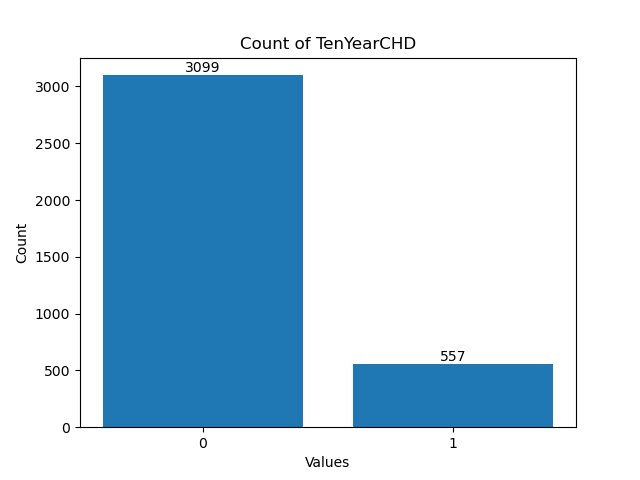
\includegraphics[width=0.5\linewidth]{Project Final/freq initial TenYearCHD.png}
    \caption{Count of TenYearCHD}
    \label{fig:Dataset List}
\end{figure}
\subsection{Dataset}
See Figure 2.
\begin{figure}[h]
    \centering
    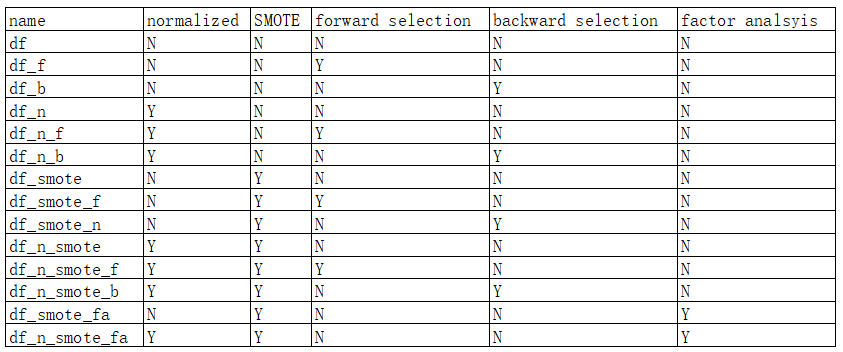
\includegraphics[width=1\linewidth]{Project Final/DATASET.png}
    \caption{Dataset}
    \label{fig:enter-label}
\end{figure}
\subsection{Logistic Regression}\\
\text The coefficients of the logistic regression model can directly indicate the impact of each predictor variable on the likelihood of CHD development. Logistic regression is well-suited for binary classification tasks, such as predicting whether an individual will develop CHD or not within a specific period. It can provide clear-cut predictions based on threshold probabilities, aiding in decision-making processes related to patient care and intervention strategies. This model is instructive for non-medical staff. Users can understand the meaning of each variable coefficient through simple prompts. Based on the impact of number value, the research will use normalized data and factor analysis data in Logistic Regression method. 
\subsection{Support Vector Machines (SVM)}\\
\text SVM's ability to handle complex and high-dimensional data, its robustness against noise, and its successful applications in medical contexts for diseases like breast cancer and liver disease further support its suitability for CHD prediction. Leveraging SVM within a machine learning approach could potentially enhance predictive accuracy and generalization, making it a compelling choice for modeling the intricacies of CHD progression over an extended timeframe. SVM algorithm is based on distance, thus the research use normalized data and factor analysis data in SVM.
\subsection{Decision Trees}\\
\text Decision trees stand out as a strong machine learning method for predicting Coronary Heart Disease (CHD) over a 10-year period due to their unique combination of interpretability, ability to capture nonlinear relationships, feature importance insights, robustness to missing data, scalability, and potential for ensemble methods. Their intuitive tree-like structure allows healthcare professionals and stakeholders to easily understand the decision rules governing CHD prediction, making them invaluable for transparent risk assessment and intervention strategies. Moreover, decision trees excel at capturing complex interactions among various risk factors, which is crucial in modeling CHD development that often involves intricate relationships among predictors. Their feature importance metrics provide insights into the most influential predictors of CHD risk, guiding further research and personalized healthcare interventions. Decision trees' robustness to missing data is particularly advantageous in real-world healthcare datasets where data completeness can be challenging. Even if users cannot provide complete detection results, they can still get high-probability results from the decision tree. Additionally, ensemble techniques like Random Forest, K-Fold extend the capabilities of decision trees by addressing overfitting and enhancing prediction accuracy, making them well-suited for long-term CHD risk prediction tasks. This study will use data without normalized. 
\subsection{Evaluation Metrics}\\
\text 
K-Fold: K-Fold Cross-Validation is a technique used in machine learning to evaluate the performance of a model by splitting the dataset into K subsets (folds). The model is trained on K-1 folds and tested on the remaining fold, repeating this process K times. In this study, all machine learning models will use 5-fold cross-validation method to avoid over fitting, and measure the evaluation.  \\\\
Accuracy: Accuracy measure the proportion of correct predictions out of the total predictions made by the model. \\
\[
    \text{Accuracy} = \frac{\text{Number of Correct Predictions}}{\text{Total Number of Predictions}} \times 100
\]
Recall: Recall, also known as sensitivity or true positive rate, measures the proportion of actual positives that are correctly identified by the mode. This article's model aims to provide warnings for future populations at risk of CHD, so this study focuses on evaluating the recall value.\\
\[
    \text{Recall} = \frac{\text{True Positives}}{\text{True Positives} + \text{False Negatives}}
\]
F-1 Score: F1-Score is the harmonic mean of precision and recall, providing a balance between these two metrics. \\
\[
\text{F1 Score} = 2 \times \frac{\text{Precision} \times \text{Recall}}{\text{Precision} + \text{Recall}}
\]
ROC: ROC is a graphical representation of the performance of a classification model across various threshold values. It plots the true positive rate against the false positive rate. 
\section{Experimental Results}
\subsection{feature selection}
\text
For Forward-stepwise selection of initial data, the selected variables are: age, sysBP, male, glucose, and cigsPerDay. \\
For Backward Elimination of initial data , the selected variables are: male, age, cigsPerDay, prevalentStroke, sysBP, and glucose\\
For Forward-stepwise selection of SMOTE data, the selected variables are: age, sysBP, cigsPerDay, prevalentHyp, glucose, male, heartRate, diaBP, and education\\
For Backward Elimination of SMOTE data, the selected variables are: male, age, education, cigsPerDay, BPMeds, prevalentHyp, diabetes, sysBP, diaBP, hearRate, and glucose. \\
Based on the Evaluate Matrics vs. Factor Number (Figure 3), the number of factor is 5.\\
Based on the Performance Metrics vs. Max Decision Tree Depth (Figure 4, 5, 6), the max depth which has best performance is 14 for SMOTE dataset, 15 for SMOTE stepwise forward selection, and 16 for SMOTE backward elimination. 

\begin{figure}[h]
    \centering
    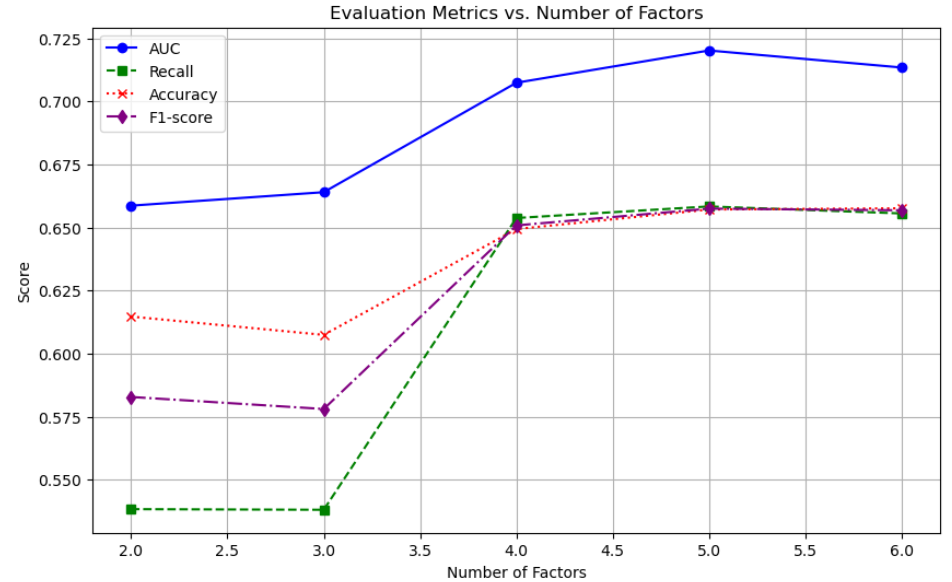
\includegraphics[width=0.5\linewidth]{Project Final/factor number.png}
    \caption{Evaluation Matrics vs. Number of Factors}
    \label{fig:enter-label}
\end{figure}
\begin{figure}[h]
    \centering
    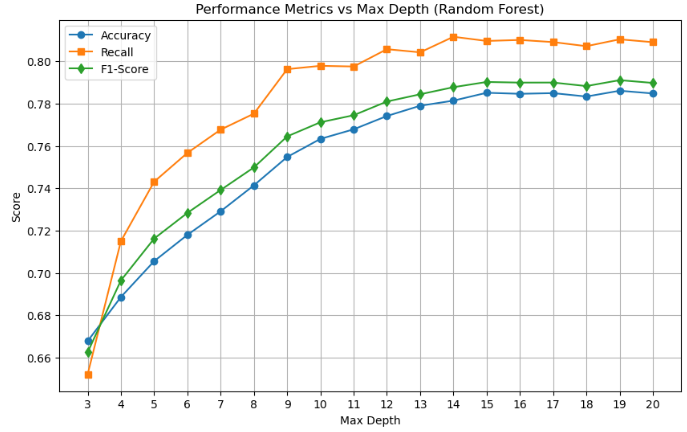
\includegraphics[width=0.5\linewidth]{Project Final/max_deep smote.png}
    \caption{Decision Tree Depth - SMOTE}
    \label{fig:enter-label}
\end{figure}
\begin{figure}[h]
    \centering
    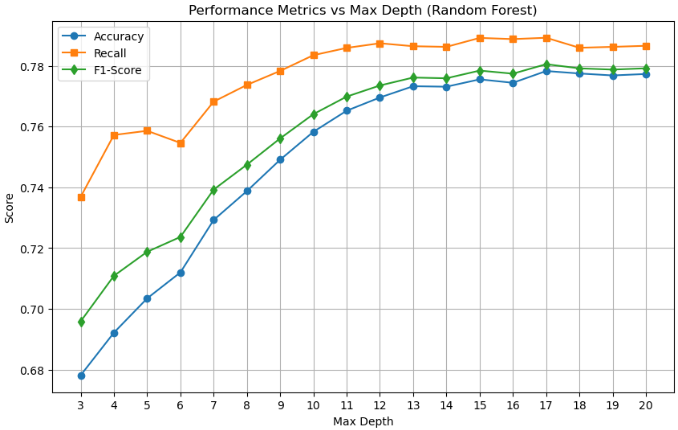
\includegraphics[width=0.5\linewidth]{Project Final/max_deep smote forward.png}
    \caption{Decision Tree Depth - SMOTE forward}
    \label{fig:enter-label}
\end{figure}
\begin{figure}[h]
    \centering
    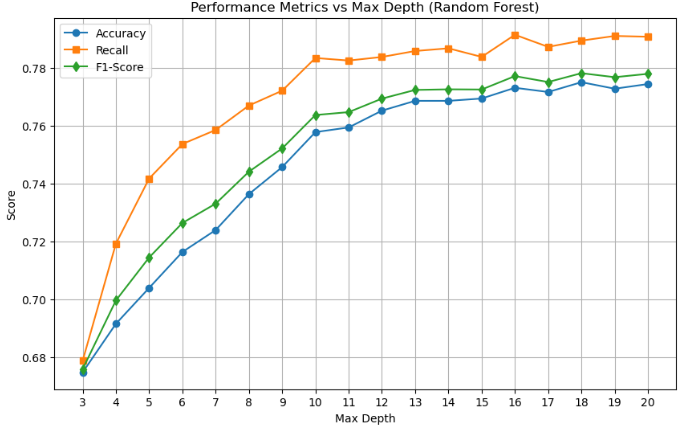
\includegraphics[width=0.5\linewidth]{Project Final/max_depth smote backward.png}
    \caption{Decision Tree Depth - SMOTE backward}
    \label{fig:enter-label}
\end{figure}
\subsection{Evaluation}
\text The accuracy, recall, and f1-score of each model are shown below (Table 1). \\
Overall, Decision Tree have better performance than Support Vector Machine. Logistic Regression performances least. The dataset without SMOTE has higher accuracy, but due to the project objection, the study wants to give a warning for high-risk people, recall of initial dataset doesn't perform well.  
\begin{table}[h]
    \centering
    \begin{tabular}{ccccc}
        Method & Dataframe  & Accuracy & Recall & F1-Score \\
        Logistic Regression & df\_n & 0.8537 & 0.0598 & 0.1097\\
        Logistic Regression & df\_n\_smote & 0.6762 & 0.6845 &0.6789 \\
        Logistic Regression & df\_n\_smote\_f & 0.6717 & 0.6786 &0.6739 \\
        Logistic Regression & df\_n\_smote\_b & 0.6736 & 0.6783 &0.6751 \\
        Logistic Regression & df\_n\_smote\_fa & 0.6593 & 0.6607 & 0.6596\\
        Support Vector Machine & df\_n& 0.8476& 0 & 0\\
        Support Vector Machine & df\_n\_smote & 0.6715 & 0.6912 & 0.6774 \\
        Support Vector Machine & df\_n\_smote\_f & 0.6717 & 0.6922 & 0.6779\\
        Support Vector Machine & df\_n\_smote\_b & 0.6741 & 0.6973 & 0.6811\\
        Support Vector Machine & df\_n\_smote\_fa & 0.6539 & 0.6696 & 0.6592\\
        Decision Tree with Random Forest (max depth = 14)& df\_smote & 0.7814 & 0.8116 & 0.7877\\
        Decision Tree with Random Forest (max depth = 15)& df\_smote\_f & 0.7756 & 0.7892 & 0.7785\\
        Decision Tree with Random Forest (max depth = 16)& df\_smote\_b & 0.7732 & 0.7915 & 0.7772\\
    \end{tabular}
    \caption{Model Evaluation}
    \label{tab:my_label}
\end{table}
\section{Conclusion}
\text 
Research has shown that BMI, as a basic classification criterion, is important for predicting the probability of getting CHD. For different BMI groups, the importance of indicators exhibited by decision trees varies. For individuals with a BMI below 22, whether they are taking medication to regulate blood pressure is crucial. In other words, for those with a BMI below 22, maintaining stable blood pressure is important. If they are taking medication to regulate blood pressure, then the variable of family history of inherited diseases becomes significant. Even though CHD is not an inherited disease, coronary heart disease has certain familial factors. This means that if you have coronary heart disease, your offspring have a higher chance of developing it in the future due to similar lifestyle habits, dietary habits, living habits, and passive smoking exposure from parents who smoke within the same family. If your BMI is around the upper limit of the normal range, even slightly higher than the normal upper limit, the probability of getting CHD will decrease. Reading through the entire model, the probability of young people getting CHD is slightly higher than that of older people. This also supports the research by Pekka Jousilahti and others in 1999.
\section{References}
\bibliographystyle{plain}
\bibliography{reference}
\nocite{*}
\end{document}
